% Autor: Simon May
% Datum: 2017-10-05
% Diese Datei bietet ein minimalistisches Grundgerüst für ein LaTeX-Dokument,
% z.B. für die Bearbeitung der Aufgaben.
\documentclass[
	% Papierformat
	a4paper,
	% Schriftgröße (beliebige Größen mit „fontsize=Xpt“)
	12pt,
	% Schreibt die Papiergröße korrekt ins Ausgabedokument
	pagesize,
	% Sprache für z.B. Babel
	ngerman
]{scrartcl}

% Achtung: Die Reihenfolge der Pakete kann (leider) wichtig sein!
% Insbesondere sollten (so wie hier) babel, fontenc und inputenc (in dieser
% Reihenfolge) als Erstes und hyperref und cleveref (Reihenfolge auch hier
% beachten) als Letztes geladen werden!

% Silbentrennung etc.; Sprache wird durch Option bei \documentclass festgelegt
\usepackage{babel}
% Verwendung der Zeichentabelle T1 (Sonderzeichen etc.)
\usepackage[T1]{fontenc}
% Legt die Zeichenkodierung der Eingabedatei fest, z.B. UTF-8
\usepackage[utf8]{inputenc}
% Schriftart
\usepackage{lmodern}
% Zusätzliche Sonderzeichen
\usepackage{textcomp}

% Mathepaket (intlimits: Grenzen über/unter Integralzeichen)
\usepackage[intlimits]{amsmath}
% Ermöglicht die Nutzung von \SI{Zahl}{Einheit} u.a.
\usepackage{siunitx}
% Zum flexiblen Einbinden von Grafiken (\includegraphics)
\usepackage{graphicx}
% Abbildungen im Fließtext
\usepackage{wrapfig}
% Abbildungen nebeneinander (subfigure, subtable)
\usepackage{subcaption}
% Funktionen für Anführungszeichen
\usepackage{csquotes}
% Zitieren, Bibliographie
\usepackage{biblatex}

% Verlinkt Textstellen im PDF-Dokument
\usepackage[unicode]{hyperref}
% "Schlaue" Referenzen (nach hyperref laden!)
\usepackage{cleveref}

% siunitx: Deutsche Ausgabe, Messfehler getrennt mit ± ausgeben
\sisetup{
	locale=DE,
	separate-uncertainty
}

\begin{document}
\begin{titlepage}
	\centering
	{\scshape\LARGE Versuchsbericht zu \par}
	\vspace{1cm}
	{\scshape\huge O4 - Magneto-Optischer-Kerr-Effekt \par}
	\vspace{2.5cm}
	{\LARGE Gruppe 6 Mo\par}
	\vspace{0.5cm}
	{\large Nils Kulawiak (E-Mail: n\_kula01@wwu.de) \par}
	{\large Oliver Brune (E-Mail: o\_brun02@wwu.de) \par}
	{\large Anthony Pietz (E-Mail: a\_piet09@wwu.de) \par}
	\vfill
	durchgeführt am 11.06.2019\par
	
	\vfill
	betreut von Christoph Angrick
	{\large \today\par}
\end{titlepage}

\tableofcontents
		
\newpage

\section{Theorie}
In der Physik spielen Oberflächen für die Eigenschaften von Stoffen eine große Rolle. Eine Methode, um die Beschaffenheit von Oberflächen genauer zu untersuchen, ist die Rastertunnelmikroskopie (eng. scanning tunneling mikroskopy, kurz: STM). Die STM gehört zu den Techniken der Rastersondenmikroskopie und basiert auf dem  quantenmechanischen Tunneleffekt. Dieser ermöglicht es Elektronen eine Potentialbarriere zwischen zwei Leitern zu durchdringen, obwohl die Barriere höher ist als die Energie des Elektrons. Im STM entspricht die Potentialbarriere dem Abstand zwischen der Spitze des Mikroskops und der zu untersuchenden Probe. Wird eine Spannung zwischen Spitze und Probe angelegt, fließt daher ein kleiner Tunnelstrom. Der einfachste Fall ist der einer rechteckigen Potentialbarriere, durch die ein freies Elektron tunnelt. Die Tunnelwahrscheinlichkeit ist für diesen Fall durch

\begin{equation}
	T(E) \approx \exp [-\frac{2}{\hbar}\sqrt{2m(\phi - E)}s]
\end{equation}

gegeben, wobei $s$ die Dicke der Potentialbarriere, $E$ die Energie des Elektrons und $\phi$ die Höhe der Potentialbarriere darstellt. Diese Gleichung lässt sich auf den allgemeinen Fall einer beliebig geformten Potentialbarriere verallgemeinern. Dann ergibt eine WKB-Näherung für den Fall, dass das Potential im Vergleich zur Wellenlänge des Elektrons langsam variiert, folgende Gleichung:

\begin{equation}
	T(E) = \exp [-\frac{2}{\hbar} \int_{z_1}^{z_2}\sqrt{2m(\phi(z) - E)}dz].
\end{equation}

Im Fall der STM tunnelt allerdings kein freies Elektron durch eine Barriere, sondern die Elektronen sind im Metall gebunden und Tunnel von einem Metall ins andere. Das dazugehörige Potential ist in \cref{barrier} gezeigt. Deshalb werden nicht mehr die Energien der freien Elektronen, sondern die Fermi-Niveaus ($E_F$) der Spitze und der Probe betrachtet. Diese sind gegeneinander verschoben, da zwischen Spitze und Probe eine Spannung angelegt wird. Ist diese positiv, liegt das Fermi-Potential der Spitze höher als das der Probe, daher tunneln die Elektronen von der Spitze zur Probe. Bei negativer Spannung ist es andersherum. Außerdem ist die Potentialbarriere abhängig von den Austrittsarbeiten der Metalle von Probe und Spitze, die in der Regel unterschiedlich sind. Zuletzt besteht auch eine Abhängigkeit von an Probe und Spitze entstehenden Bildladungen.

\begin{figure}[h!]
	\centering
	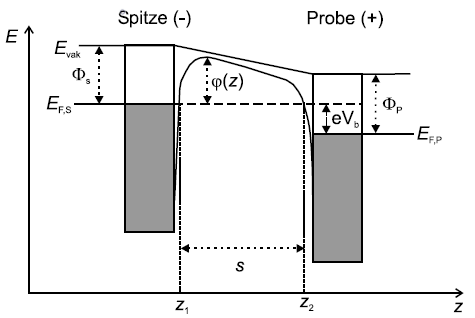
\includegraphics[scale = 1.2]{barrier.png}
	\caption{Die Grafik zeigt die Potentialbarriere zwischen Spitze und Probe im STM. Aufgrund der Tunnelspannung sind die beiden Fermi-Niveaus gegeneinander verschoben. Da die angelegte Spannung hier positiv ist, fällt die Potentialbarriere zwischen Spitze und Probe linear ab. Für die Abrundung des Potentials an den Rändern sind Bildladungen verantwortlich.}
	\label{barrier}
\end{figure}

Um nun die Oberfläche des zu untersuchenden Stoffes abzubilden, wird die Spitze des STM in $x$- und $y$-Richtung über die Probe gefahren. Dabei wird für jede Einstellung der Tunnelstrom gemessen. Es gibt zwei verschiedene Messmodi: Einerseits ist es möglich, den Abstand zur Probe konstant zu halten, dann wird aus der Änderung des Tunnelstroms die Beschaffenheit der Oberfläche bestimmt. Zum anderen kann auch der Tunnelstrom konstant gehalten werden, indem mithilfe eines Regelkreises der Probenabstand entsprechend variiert wird. In diesem Versuch wurde die zweite Möglichkeit verwendet. Das STM erstellt somit ein Höhenprofil der Oberfläche. Die Höhe der Oberfläche entspricht dabei der lokalen Elektronenzustandsdichte. Dieses Profil kann atomgenau erstellt werden, da der Tunneleffekt auf sehr kleinen Abständen stattfindet und er bereits von Abstandsänderungen von weniger als $\SI{1}{\angstrom}$ beeinflusst wird. Daher ist es notwendig, dass die Spitze des Mikroskops sehr fein ist, im Optimalfall besteht sie nur aus einem einzelnen Atom, von dem die Elektronen in die Probe tunneln können. Außerdem wird für die Bestimmung des Höhenprofils der Tunnelstrom benötigt. Hierfür ist ein Modell nötig, das im folgenden eingeführt wird.

\subsection{Tersoff-Hamann-Modell}
Bei einer vollständigen dreidimensionalen Berechnung des Tunnelstroms ergibt sich eine komplizierte, analytisch nicht lösbare Gleichung, sodass nur mit hohem Rechenaufwand ein Ergebnis bestimmt werden könnte. Zur Vereinfachung stellten J. Tersoff und D.R. Hamann im Jahr 1985 ein vereinfachtes Modell vor, mit dem der Tunnelstrom genähert werden kann. Dieses Modell ist nach ihren Erfindern als Tersoff-Hamann-Modell bekannt. Hierbei wird der Tunnelstrom mithilfe der zeitabhängigen Störungstheorie erster Ordnung berechnet. Das Modell geht davon aus, dass sich an der Spitze des Mikroskops nur ein einzelnes Atom mit sphärischer Oberfläche befindet ,und dass die Probe eben ist (siehe \cref{spitze}).

\begin{figure}[h!]
	\centering
	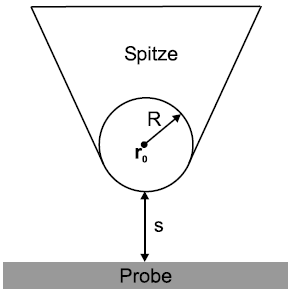
\includegraphics[scale=0.8]{spitze.png}
	\label{spitze}
	\caption{Der Tunnelkontakt nach dem Tersoff-Hamann-Modell. Die Annahmen des einzelnen Atoms an der Spitze mit Krümmungsradius $R$ und der ebenen Probe sind hier dargestellt.}
\end{figure}

In der ersten Ordnung Störungstheorie, die hier verwendet wird, ergibt sich für den Tunnelstrom
\begin{equation}
	I = \frac{2\pi e}{\hbar} \sum_{\mu, \nu} |M_{\mu,\nu}|^2 f(E_\mu)[1-f(E_\nu + eV_b)] \delta(E_\mu - E_\nu),
	\label{eq:I1}
\end{equation}
wobei $E_\mu$ und $E_\nu$ die Energien der Zustände der Spitze bzw. Probe und $f$ die Fermi-Dirac-Verteilungsfunktion für die Zustände der Spitze ($\mu$) und der Probe ($\nu$) bezeichnet. $V_\text{b}$ ist die angelegte Spannung zwischen Spitze und Probe. Die Delta-Funktion sorgt dafür, dass nur elastische Tunnelprozesse betrachtet werden. $M_{\mu,\nu}$ ist das Matrixelement, dass den Übergang zwischen den Zuständen von Spitze und Probe beschreibt. Diese Gleichung lässt sich mit einigen simplen Annahmen deutlich vereinfachen. Nimmt man niedrige Temperatur und kleine Tunnelspannungen an, erhält man
\begin{equation}
	I = \frac{2\pi e^2}{\hbar}V_\text{b} \sum_{\mu, \nu} |M_{\mu,\nu}|^2 \delta(E_\mu - E_\text{F}) \delta(E_\nu - E_\text{F}),
	\label{eq:I2}
\end{equation}
mit der Energie des Fermi-Niveaus $E_\text{F}$.

Eine Möglichkeit zur Bestimmung des Matrixelements entwickelte John Bardeen im Jahr 1961. \cite{1} Die von ihm entdeckte Gleichung lautet

\begin{equation}
	M_{\mu,\nu} = \frac{\hbar^2}{2m_\text{e}} \int_{\text{d}S} \text{d}S(\Psi_\mu^* \nabla \Psi_\nu - \Psi_\nu \nabla \Psi_\mu^*).
	\label{eq:M}
\end{equation}
$\Psi_\mu$ und $\Psi_\nu$ sind die Zustände der Spitze bzw. der Probe. Der Ausdruck in der Klammer entspricht dem quantenmechanischen Stromdichteoperator. Integriert wird über $S$, dies ist eine Querschnittsfläche, die vollständig im Bereich zwischen den Elektroden liegt, also Spitze und Probe voneinander trennt. Um das Übergangsmatrixelement zu berechnen, müssen nun noch $\Psi_\mu$ und $\Psi_\nu$ bestimmt werden. Die Wellenfunktion der Spitze wird durch eine s-Wellenfunktion der Form

\begin{equation}
	\Psi_\mu = \frac{1}{\sqrt{V_\text{S}}} R \exp(\kappa R) \frac{1}{|r-r_0|} \exp(-\kappa|r-r_0|)
	\label{eq:psimu}
\end{equation}

beschrieben, wobei $V_\text{s}$ das Volumen der Spitze, $R$ den Krümmungsradius, $r_0$ die Position des Mittelpunktes des Spitzenendes, $\kappa = \frac{\sqrt{2m_\text{e}\Phi}}{\hbar}$ die inverse Abklinglänge der Welle im Vakuum und $\Phi$ die Austrittsarbeit beschreibt. Die Wellenfunktion der Probe ist durch

\begin{equation}
	\Psi_\nu = \frac{1}{\sqrt{V\text{P}}} \sum_{G} a_G \exp(-\sqrt{\kappa^2 + |k_\parallel + G|^2}z) \exp[i(G + k_\parallel)]
	\label{eq:psinu}
\end{equation}

gegeben mit Volumen der Probe $V_\text{P}$, einem reziproken Gittervektor $G$ mit Entwicklungskoeffizient $a_G$ und dem zur Oberfläche parallelen Teil des Bloch-Wellenvektor $k_\parallel$.
Zur Vereinfachung werden die Austrittsarbeiten von Spitze und Probe als gleich angenommen. Indem \cref{eq:psimu} und \cref{eq:psinu} in \cref{eq:M} und diese anschließend in \cref{eq:I2} eingesetzt werden, erhält man als Endergebnis

\begin{equation}
	I = \frac{32 \pi^3 e^2}{\hbar} V_{\text{b}} \frac{\Phi^2}{\kappa^4} \rho_\text{S}(E_\text{F}) R^2 \exp(2 \kappa R) \rho_\text{P}(r_0, E_\text{F}).
	\label{eq:I3}
\end{equation}

Hierbei sind $\rho_\text{S}(E_\text{F})$ die normierte Zustandsdichte der Spitze und $\rho\text{P}(r_0, E_\text{F}) = \sum_{\nu} |\Psi_\nu(r_0)|^2 \delta(E_\nu - E_\text{F})$ die lokale Zustandsdichte der Probe.

Aus \cref{eq:I3} ergeben sich einige wichtige Eigenschaften des Tunnelstroms im STM. Der Tunnelstrom hängt exponentiell vom Abstand zwischen Spitze und Probe ab.
Wird der Tunnelstrom während der Messung konstant gehalten, variiert die Höhe der Spitze je nach elektronischer Struktur der Probe an dieser Stelle. Diese Abhängigkeit von der lokalen Zustandsdichte am Fermi-Niveau ermöglicht es, auf diese Weise die Topographie der Probe zu kartographieren. Diese enthält Informationen darüber, um welchen Stoff es sich handelt und wie die Atome im Gitter sortiert sind. Außerdem können Korngrenzen und Defekte im Kristallgitter identifiziert werden.

Um ein möglichst genaues Ergebnis zu erhalten, muss das Auflösungsvermögen maximiert werden. Dies wurde abgeschätzt auf

\begin{equation}
	2\rho = 1,66 \sqrt{\frac{R + s}{\kappa}}
	\label{eq:sigma}
\end{equation}

Um eine möglichst gute Messung durchzuführen, sollten also an der Spitze des Rastertunnelmikroskops nur ein einzelnes Atom sitzen. Außerdem sollte der Abstand zwischen Spitze und Probe so klein wie möglich sein.

Mit diesem Modell lässt sich die Theorie hinter dem Rastertunnelmikroskop bereits gut erklären, gleichzeitig ist es aber auch noch mit relativ einfachen Mitteln berechenbar. Für eine genauere Berechnung wären weitere Informationen über die Wellenfunktion der Spitze nötig. Außerdem ließe sich ein komplexeres Modell nicht mehr auf eine einfache Formel reduzieren.

\newpage

\begin{thebibliography}{9}
	\bibitem{A}
	J. Bardeen, Phys. Rev. Lett. 6, 57 (1961).
	\bibitem{B}
	J. Tersoff, D. R. Hamann, Phys. Rev. Lett. 50, 1998 (1983)
\end{thebibliography}
\end{document}